\documentclass[margin,line]{resume}
 
\usepackage[utf8]{inputenc}
\usepackage[english]{babel}
\usepackage[T1]{fontenc}
\usepackage{fontawesome}
\usepackage{graphicx,wrapfig}
\usepackage{url}
\usepackage[colorlinks=true, pdfstartview=FitV, linkcolor=blue, citecolor=blue, urlcolor=blue]{hyperref}
\ifdefined\pdfcompresslevel
\pdfcompresslevel=9
\fi


\begin{document}{\sc \Large Curriculum Vitae -- Arthur Guiot}
\begin{resume}

% === PICTURE ===

    \vspace{0.5cm}
    \begin{wrapfigure}{R}{0.15\textwidth}
         \vspace{-1.5cm}
        \begin{center}
        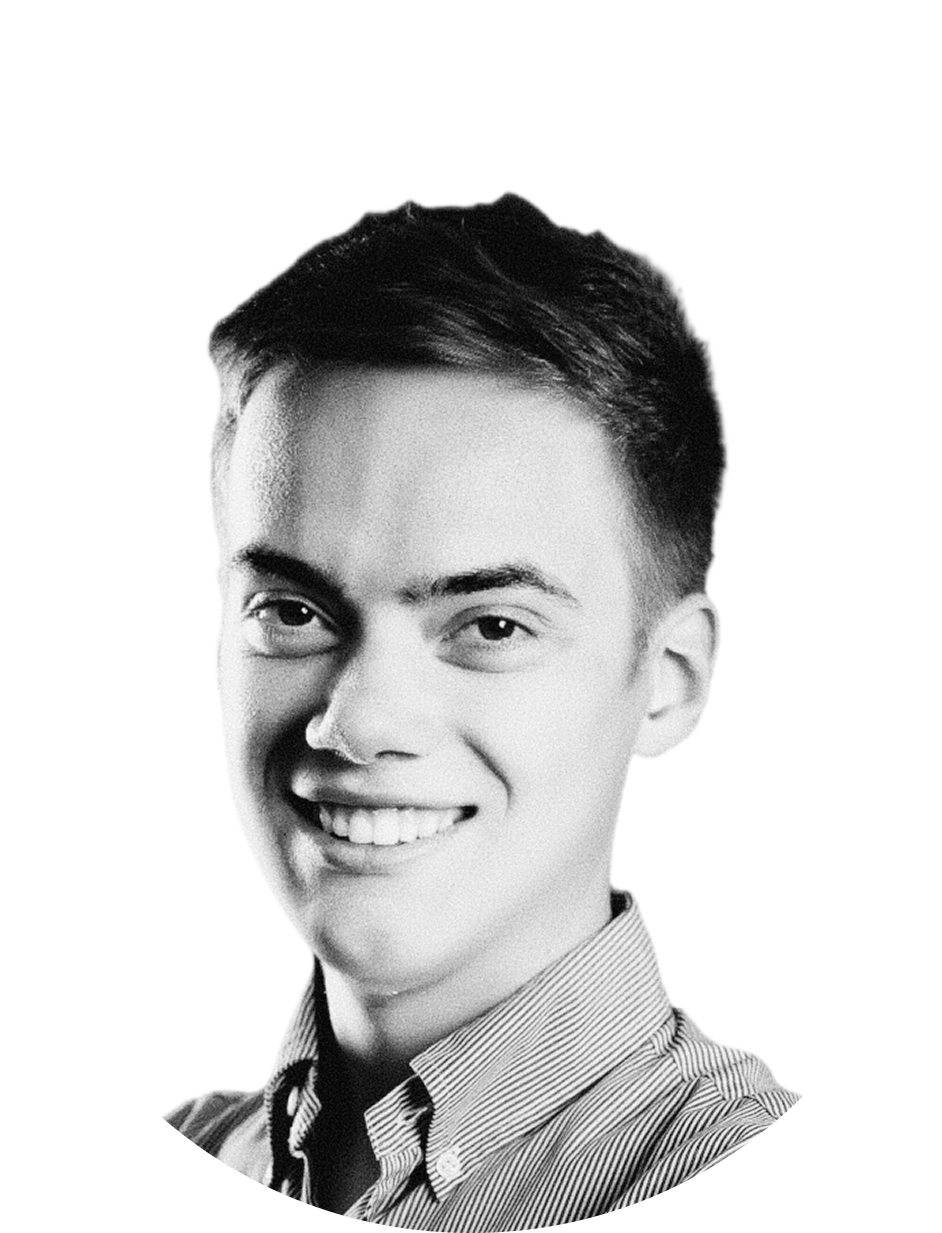
\includegraphics[width=0.15\textwidth]{profile_picture.png}
        \end{center}
         \vspace{-1cm}
    \end{wrapfigure}

% === PERSONAL INFO ===
 
    \section{\mysidestyle Personal\\Information}
    Arthur Guiot \\
    Santa Clara, California, USA \\ 
    \faPhone \space +1 (863) 210-4074 \\
    \faEnvelope \space \href{mailto:arguiot@gmail.com}{arguiot@gmail.com} \\ 
    \faGlobe \space \href{https://arguiot.com}{arguiot.com} \\ 
    \faGithub \space \href{https://github.com/arguiot}{github.com/arguiot} \\
    Active open-source contributor with 7,500+ contributions and 2,000+ stars on GitHub
   
% === OBJECTIVE ===

    \section{\mysidestyle Professional Objective}
    Software engineering student with 8 years of experience in application development, website optimization, and blockchain technology. Seeking to leverage technical expertise in developing high-performance financial applications and distributed systems to drive innovation in the technology and finance sectors.
 
% === SKILLS ===
       
    \section{\mysidestyle Skills}\vspace{2mm}       
    \begin{description}
        \item[User Facing:] Next.js, Tailwind, React, SwiftUI, UIKit, AppKit
        \item[Business Logic:] TypeScript, Python, Swift, C \& C++, SQL, Solidity, Rust
        \item[Other Technologies:] Git, Linux, AWS, Kubernetes, DevOps, Docker
        \item[Professional Skills:] Leadership, Project Management, Client Communication, Fund raising
        \item[Languages:] French, English
    \end{description}
     
% === FEATURED PROJECTS ===
    
    \section{\mysidestyle Featured Projects}
    \begin{list2}
        \item \textbf{Euclid Calculator}\\
        A completely redesigned calculator for macOS and iOS with a 4.5-star rating across countries. Recommended by SetApp, with over 50K paid downloads across platforms.
        \vspace{1mm}
        \item \textbf{Ultrahuman}\\
        A fully autonomous support system that helps debug tickets by spawning agents to inspect codebases and systems, accelerating root-cause analysis across product and infrastructure issues.
        \vspace{1mm}
        \item \textbf{Portfolio Manager}\\
        Automatic crypto portfolio management system that grew from 0 to \$100K AUM within three months of deployment. Features extensive backtesting capabilities for finance and quantitative models serving hundreds of clients.
    \end{list2}

% === EDUCATION ===

\section{\mysidestyle Education} 
\textbf{Santa Clara University, California} \hfill \textsl{September 2023-June 2025}\\
Bachelor of Computer Science\\
\vspace{1mm}
\textbf{Florida Polytechnic University, Florida} \hfill \textsl{January 2021-September 2023}\\
Bachelor of Computer Science (transferred to SCU)
    
% === EMPLOYMENT HISTORY ===

    \section{\mysidestyle Experience}\vspace{2mm}   	   
       
    \begin{description} 
        \item[Software Engineer]\small{Circleback \hfill \textsl{July 2026-Present}}\\
        Achievements:
        \begin{list2}
            \item{Working full-time at Circleback, a YC-backed AI meeting notes company}
            \item{Building products that help teams capture, organize, and act on meeting conversations more effectively}
            \item{Contributing across product engineering for AI-powered workflows and meeting productivity tools}
        \end{list2}
        \vspace{2mm}

        \item[Blockchain Engineer]\small{EveryFinance \hfill \textsl{January 2024-March 2025}}\\
        Achievements:
        \begin{list2}
            \item{Built financial tools and backtesting framework generating 85\% APR (averaged across 5 years) for the Alpha portfolio}
            \item{Reduced processing times from 5-15 seconds to 1-3 seconds, significantly improving UX}
            \item{Centralized infrastructure state across 20+ microservices and implemented CI system}
        \end{list2}   	
        \vspace{2mm}
 				
        \item[Blockchain Engineer Intern]\small{PyratzLabs \hfill \textsl{May 2023-August 2023}}\\
        Achievements:
        \begin{list2}
            \item{Designed and built an arbitrage bot with theoretical potential profits of 75 ETH per week based on internal research}
            \item{Worked on a portfolio optimization tool that informed investment strategy decisions}
            \item{Helped build Securd, a revolutionary lending \& borrowing protocol on Ethereum chains}
        \end{list2}  	      
        \vspace{2mm}
    \end{description}
    
\end{resume}   
\end{document}
